\documentclass[
  man,
  floatsintext,
  longtable,
  nolmodern,
  notxfonts,
  notimes,
  colorlinks=true,linkcolor=blue,citecolor=blue,urlcolor=blue]{apa7}

\usepackage{amsmath}
\usepackage{amssymb}



\usepackage[bidi=default]{babel}
\babelprovide[main,import]{english}


% get rid of language-specific shorthands (see #6817):
\let\LanguageShortHands\languageshorthands
\def\languageshorthands#1{}

\RequirePackage{longtable}
\RequirePackage{threeparttablex}

\makeatletter
\renewcommand{\paragraph}{\@startsection{paragraph}{4}{\parindent}%
	{0\baselineskip \@plus 0.2ex \@minus 0.2ex}%
	{-.5em}%
	{\normalfont\normalsize\bfseries\typesectitle}}

\renewcommand{\subparagraph}[1]{\@startsection{subparagraph}{5}{0.5em}%
	{0\baselineskip \@plus 0.2ex \@minus 0.2ex}%
	{-\z@\relax}%
	{\normalfont\normalsize\bfseries\itshape\hspace{\parindent}{#1}\textit{\addperi}}{\relax}}
\makeatother




\usepackage{longtable, booktabs, multirow, multicol, colortbl, hhline, caption, array, float, xpatch}
\setcounter{topnumber}{2}
\setcounter{bottomnumber}{2}
\setcounter{totalnumber}{4}
\renewcommand{\topfraction}{0.85}
\renewcommand{\bottomfraction}{0.85}
\renewcommand{\textfraction}{0.15}
\renewcommand{\floatpagefraction}{0.7}

\usepackage{tcolorbox}
\tcbuselibrary{listings,theorems, breakable, skins}
\usepackage{fontawesome5}

\definecolor{quarto-callout-color}{HTML}{909090}
\definecolor{quarto-callout-note-color}{HTML}{0758E5}
\definecolor{quarto-callout-important-color}{HTML}{CC1914}
\definecolor{quarto-callout-warning-color}{HTML}{EB9113}
\definecolor{quarto-callout-tip-color}{HTML}{00A047}
\definecolor{quarto-callout-caution-color}{HTML}{FC5300}
\definecolor{quarto-callout-color-frame}{HTML}{ACACAC}
\definecolor{quarto-callout-note-color-frame}{HTML}{4582EC}
\definecolor{quarto-callout-important-color-frame}{HTML}{D9534F}
\definecolor{quarto-callout-warning-color-frame}{HTML}{F0AD4E}
\definecolor{quarto-callout-tip-color-frame}{HTML}{02B875}
\definecolor{quarto-callout-caution-color-frame}{HTML}{FD7E14}

%\newlength\Oldarrayrulewidth
%\newlength\Oldtabcolsep


\usepackage{hyperref}




\providecommand{\tightlist}{%
  \setlength{\itemsep}{0pt}\setlength{\parskip}{0pt}}
\usepackage{longtable,booktabs,array}
\usepackage{calc} % for calculating minipage widths
% Correct order of tables after \paragraph or \subparagraph
\usepackage{etoolbox}
\makeatletter
\patchcmd\longtable{\par}{\if@noskipsec\mbox{}\fi\par}{}{}
\makeatother
% Allow footnotes in longtable head/foot
\IfFileExists{footnotehyper.sty}{\usepackage{footnotehyper}}{\usepackage{footnote}}
\makesavenoteenv{longtable}

\usepackage{graphicx}
\makeatletter
\def\maxwidth{\ifdim\Gin@nat@width>\linewidth\linewidth\else\Gin@nat@width\fi}
\def\maxheight{\ifdim\Gin@nat@height>\textheight\textheight\else\Gin@nat@height\fi}
\makeatother
% Scale images if necessary, so that they will not overflow the page
% margins by default, and it is still possible to overwrite the defaults
% using explicit options in \includegraphics[width, height, ...]{}
\setkeys{Gin}{width=\maxwidth,height=\maxheight,keepaspectratio}
% Set default figure placement to htbp
\makeatletter
\def\fps@figure{htbp}
\makeatother







\usepackage{newtx}

\defaultfontfeatures{Scale=MatchLowercase}
\defaultfontfeatures[\rmfamily]{Ligatures=TeX,Scale=1}





\title{The relationship between international study and civic virtues}


\shorttitle{The relationship between international study and civic
virtues}


\usepackage{etoolbox}






\author{Yangyue Li}



\affiliation{
{MA Program in the Social Sciences, University of Chicago}}




\leftheader{Li}



\abstract{Not ready}

\keywords{civic virtues, empathy, wisdom, civility}

\authornote{ 

\par{       }
\par{Correspondence concerning this article should be addressed
to Yangyue Li, MA Program in the Social Sciences, University of
Chicago, 1155 E 60th
St., Chicago, IL 60637, USA, Email: yangyueli28@uchicago.edu}
}

\makeatletter
\let\endoldlt\endlongtable
\def\endlongtable{
\hline
\endoldlt
}
\makeatother

\urlstyle{same}



\usepackage{booktabs}
\usepackage{longtable}
\usepackage{array}
\usepackage{multirow}
\usepackage{wrapfig}
\usepackage{float}
\usepackage{colortbl}
\usepackage{pdflscape}
\usepackage{tabu}
\usepackage{threeparttable}
\usepackage{threeparttablex}
\usepackage[normalem]{ulem}
\usepackage{makecell}
\usepackage{xcolor}
\makeatletter
\@ifpackageloaded{caption}{}{\usepackage{caption}}
\AtBeginDocument{%
\ifdefined\contentsname
  \renewcommand*\contentsname{Table of contents}
\else
  \newcommand\contentsname{Table of contents}
\fi
\ifdefined\listfigurename
  \renewcommand*\listfigurename{List of Figures}
\else
  \newcommand\listfigurename{List of Figures}
\fi
\ifdefined\listtablename
  \renewcommand*\listtablename{List of Tables}
\else
  \newcommand\listtablename{List of Tables}
\fi
\ifdefined\figurename
  \renewcommand*\figurename{Figure}
\else
  \newcommand\figurename{Figure}
\fi
\ifdefined\tablename
  \renewcommand*\tablename{Table}
\else
  \newcommand\tablename{Table}
\fi
}
\@ifpackageloaded{float}{}{\usepackage{float}}
\floatstyle{ruled}
\@ifundefined{c@chapter}{\newfloat{codelisting}{h}{lop}}{\newfloat{codelisting}{h}{lop}[chapter]}
\floatname{codelisting}{Listing}
\newcommand*\listoflistings{\listof{codelisting}{List of Listings}}
\makeatother
\makeatletter
\makeatother
\makeatletter
\@ifpackageloaded{caption}{}{\usepackage{caption}}
\@ifpackageloaded{subcaption}{}{\usepackage{subcaption}}
\makeatother

% From https://tex.stackexchange.com/a/645996/211326
%%% apa7 doesn't want to add appendix section titles in the toc
%%% let's make it do it
\makeatletter
\xpatchcmd{\appendix}
  {\par}
  {\addcontentsline{toc}{section}{\@currentlabelname}\par}
  {}{}
\makeatother

%% Disable longtable counter
%% https://tex.stackexchange.com/a/248395/211326

\usepackage{etoolbox}

\makeatletter
\patchcmd{\LT@caption}
  {\bgroup}
  {\bgroup\global\LTpatch@captiontrue}
  {}{}
\patchcmd{\longtable}
  {\par}
  {\par\global\LTpatch@captionfalse}
  {}{}
\apptocmd{\endlongtable}
  {\ifLTpatch@caption\else\addtocounter{table}{-1}\fi}
  {}{}
\newif\ifLTpatch@caption
\makeatother

\begin{document}

\maketitle


\setcounter{secnumdepth}{-\maxdimen} % remove section numbering

\setlength\LTleft{0pt}


In an interconnected world, civic virtues are crucial for fostering
responsible citizenship and encouraging individuals to prioritize
societal well-being over self-interest (Sherrod et al., 2002). U.S.
universities, as diverse microcosms, bring domestic and international
students together, offering unique contexts for civic engagement and
understanding the values of others. Domestic American students may
develop civic engagement through strong ties to their local communities
and the American education system, while international students may
bring perspectives shaped by cross-cultural experiences and adaptation
to a new cultural environment. Undergoing the same admission process and
sharing similar college life on campus with their American peers,
international students may still differ in civic behaviors. These
contexts raise critical questions about the factors that foster civic
virtues and motivate individuals to engage in civic-minded behaviors.
How do experiences in a foreign and culturally different environment
influence civic virtues and related psychological characteristics such
as empathy and cultural competence? Do international students differ on
these psychological aspects from US students?

\subsection{Literature Review}\label{literature-review}

\subsubsection{Education and Civic
Virtues}\label{education-and-civic-virtues}

Civic engagement may foster a sense of belonging, purpose, and
responsibility within a community, and may empower individuals to
contribute to a common good (Flanagan \& Levine, 2010). Research
suggests that civic education - educational experiences that are
directed at increasing civic virtues - happens mostly during
adolescence, but can continue into young adulthood (Flanagan \& Levine,
2010; Sherrod et al., 2002). Much of this experience occurs in
educational settings, particularly colleges, which offer structured
opportunities through coursework, extracurricular activities, community
service programs, and student organizations (Flanagan \& Levine, 2010).
These experiences could help young adults develop civic virtues and
social responsibility.

Besides formal instruction in character education and civility (Jeynes,
2019; Torney-Purta, 2002), non-didactic and informal experiences have
important implications for the development of civic virtues as well.
Indeed, research highlights that youths who are involved in
community-based organizations or extracurricular activities are more
likely to be civically active (Zarrett et al., 2021). Furthermore, a
study suggests that participating in community service or volunteering
is associated with adolescent civic beliefs about considering similar
types of civic engagement behaviors (Metzger et al., 2019). Similarly,
Vazina \& Poulin (2019) found that prosocial/community-based activities
are related to a greater likelihood of being in the high-sustained civic
engagement trajectory.

Additionally, recent research suggests that study abroad programs may
increase some aspects of civic virtues and related psychological
capacities. Living and studying in a foreign cultural environment
provide opportunities for students to interact with people from diverse
backgrounds, fostering skills related to civic virtues such as empathy,
open-mindedness, and perspective-taking in a non-didactic way (Chieffo
\& Griffiths, 2004). Research indicates that even short-term study
abroad programs enhance student's empathy and open-mindedness toward
diverse perspectives, and foster a deeper sense of responsibility as
global citizens (Chieffo \& Griffiths, 2004). Black and Duhon (2006)
assessed the impact of a month-long business-focused study abroad
program in London on students' cultural awareness and personal
development. Consistent with previous findings, students showed
significant improvements in cross-cultural empathy and understanding of
global perspectives. A more recent study examined the relationship
between studying abroad and civic virtues (Boulware et al., 2023). The
results suggest that undergraduate students who have gone abroad via one
particular set of study abroad programs in undergraduate studies
demonstrated higher levels of empathy, civic engagement, and civility
toward others, compared with students who do not have these experiences
or have no interest in them.

\subsubsection{Current Study}\label{current-study}

The study examined how factors such as international students' first
language, English language fluency, and the duration of their residence
in the United States relate to civic virtues. We hypothesize that
international students with greater English fluency and who live in the
United States for a longer period of time will score higher on civic
virtues, as students with higher fluency may feel more confident and
able to engage in community activities and social settings. However, it
is unclear whether different native languages would interact with this.
Given that language differences are related to cultural differences, it
may be the case that English competence alone may not be significant. We
hypothesize that non-English-native speakers may score higher on civic
virtues than students who are native or heritage bilingual speakers of
English, maybe because navigating a foreign environment in a non-native
language may require greater effort and adaptation, fostering civic
virtues. Additionally, we also examined the possible interaction between
first language and English fluency to investigate whether non-native
English speakers who are more fluent in English score the highest civic
virtues.

\section{Method}\label{method}

\subsection{Participants}\label{participants}

\begin{table}

{\caption{{Demographic Characteristics of
Participants}{\label{tbl-demographics}}}
\vspace{-20pt}}

\begin{longtable*}[t]{llll}
\toprule
Label & Level & American & International\\
\midrule
Age (years) & Mean (SD) & 19.39 (0.89) & 19.77 (1.10)\\
Gender & Female & 38 (67.9\%) & 14 (46.7\%)\\
 & Male & 17 (30.4\%) & 14 (46.7\%)\\
 & Prefer not to answer & 1 (1.8\%) & 2 (6.7\%)\\
Ethnicity & Asian & 21 (37.5\%) & 18 (60.0\%)\\
\addlinespace
 & Black or African American & 5 (8.9\%) & NA\\
 & Not specified & 1 (1.8\%) & NA\\
 & Prefer not to answer & 2 (3.6\%) & 2 (6.7\%)\\
 & Prefer to self-describe & 2 (3.6\%) & 2 (6.7\%)\\
 & Two or more races & 6 (10.7\%) & 1 (3.3\%)\\
\addlinespace
 & White & 18 (32.1\%) & 7 (23.3\%)\\
 & NA & 1 (1.8\%) & NA\\
\bottomrule
\end{longtable*}

\end{table}

A survey was adapted from Boulware et al.~(2023). Participants were
recruited through the Psychology Department's SONA system during the
winter quarter in 2025 as well as through campus advertisements. The
total sample consisted of 86 participants, with 30 international
students and 56 domestic students, representing a diverse composition of
student backgrounds as detailed in Table~\ref{tbl-demographics}.

\subsection{Measures}\label{measures}

A survey will be adapted from Boulware et al.~(2023), and distributed
through the Psychology Department's research participant recruitment
system during the winter quarter in 2025.

\subsubsection{Civic Virtues}\label{civic-virtues}

We will use two measures to assess civic virtues. The first is Doolittle
and Faul's (2013) 14-item Civic Engagement Scale. It includes the 8
civic attitude subscale (e.g., ``I feel responsible for my community'',
1 = disagree, and 7 = agree) and 6 civic behavior items (e.g., ``I am
involved in structured volunteer position(s) in the community'', 1 =
never, and 7 = always). The second one is based on the Workplace
Relational Civility scale, tailored for student population. It includes
13 items assessing civility towards others and 13 items assessing
civility experienced by participants (Di Fabio \& Gori, 2016). Sample
items include ``I was able to express my values and my beliefs calmly to
others'' and ``Others were able to express their point of view without
being disrespectful toward me'' (1= not at all, and 5 = a great deal).

\subsubsection{Other constructs related to civic
virtues}\label{other-constructs-related-to-civic-virtues}

We will use a scale developed at the Center for Practical Wisdom at the
University of Chicago to assess epistemic humility (Hoeckner, 2011,
personal communication). Sample items include ``I accept that many good
and bad things happening to me are beyond my control'' (1 = strongly
disagree, and 8 = strongly agree). We will use the 8-item Empathy
Quotient to measure empathy towards others (Loewen et al., 2009). Sample
items include ``I find it easy to put myself in somebody else's shoes''
(1 = never, and 5 = always). We will use the 6-item NFC short form scale
to measure the tendency to engage in cognitive effort (Lins De Holanda
Coelho et al., 2020). Sample questions include ``I would prefer complex
to simple problems'' (1 = extremely uncharacteristic, and 5 = extremely
characteristic). We will measure cultural competency based on a set of
questions provided by the Study Abroad program at the University of
Chicago. For international students, we will have questions asking them
to report their first language, English proficiency (indicated by the
Test of English as a Foreign Language or a self-report scale), and
duration of their residence in the United States. American students will
indicate whether they have studied abroad.

\subsection{Data Analysis}\label{data-analysis}

To test the first hypothesis, independent t-tests will compare
international and American students on each measure of civic virtues
(civic attitudes, civic behaviors, and civility) and other related
constructs. These comparisons will indicate whether international
students, as a group, exhibit different levels of civic virtues compared
to their American peers. Given the interrelated nature of some of these
measures, a multivariate analysis of covariance (MANCOVA) will be
conducted to account for relationships among the dependent variables and
provide a more comprehensive analysis. To address the second hypothesis,
multiple regression analyses will examine the relationships between
English language proficiency, residency duration, and first language on
civic virtues within the international student population. Separate
models will be run for each dimension of civic virtues and related
measures to determine how strongly these factors are related to
different aspects of civic engagement. To address the third hypothesis,
a one-way analysis of variance (ANOVA) will be conducted to examine
differences in civic virtues among first-language groups
(English-native, non-English-native, and heritage bilinguals). Moreover,
an interaction term (First Language × English Fluency) will be included
in regression analyses to determine whether the relationship between
fluency and civic virtues varies across language groups.

\section{Results}\label{results}

\subsection{Descriptive Analyses}\label{descriptive-analyses}

\begin{table}

{\caption{{Descriptive Statistics of Civic Virtues
Measures}{\label{tbl-descriptive-stats}}}
\vspace{-20pt}}

\begin{tabular}[t]{lrrrrr}
\toprule
Variable & Mean & SD & Median & Min & Max\\
\midrule
CB\_CA Total & 72.05 & 14.34 & 72.0 & 33 & 98\\
Civic Attitudes & 43.52 & 8.51 & 43.0 & 20 & 56\\
Civic Behaviors & 28.52 & 7.18 & 28.5 & 13 & 42\\
Civility Total & 101.81 & 13.36 & 101.5 & 73 & 130\\
Civility Towards Me & 48.30 & 8.57 & 48.5 & 28 & 65\\
\addlinespace
Civility Towards Others & 53.51 & 6.86 & 53.0 & 36 & 65\\
Cultural Competence & 34.16 & 4.39 & 34.5 & 19 & 43\\
Empathy & 29.41 & 3.65 & 30.0 & 22 & 37\\
Epistemic Humility & 94.52 & 12.88 & 95.5 & 62 & 122\\
Need for Closure & 57.88 & 12.35 & 57.0 & 30 & 91\\
\addlinespace
Need for Cognition & 21.71 & 3.87 & 22.0 & 12 & 30\\
Wise Reasoning & 76.59 & 12.81 & 76.5 & 26 & 105\\
\bottomrule
\end{tabular}

\end{table}

Descriptive statistics for the key measures of civic virtues are
presented in Table~\ref{tbl-descriptive-stats}. The sample exhibited
varying levels of psychological constructs related to civic engagement.
\emph{Civic Attitudes} showed a mean of 43.52 (\emph{SD} = 8.51), with a
range from 20 to 56. \emph{Civic Behaviors} displayed a mean of 28.52
(\emph{SD} = 7.18), suggesting moderate levels of community engagement.

The variability across different civic virtue measures suggests
potential differences in how participants conceptualize and enact civic
engagement. \emph{Epistemic Humility}, for instance, ranged from 62 to
122, with a mean of 94.52 (\emph{SD} = 12.88), indicating considerable
individual variation in this construct.

\subsection{Bivariate Correlations}\label{bivariate-correlations}

\begin{table}

{\caption{{Bivariate Correlations among Civic Virtues
Constructs}{\label{tbl-correlations}}}
\vspace{-20pt}}

[!h]
\centering
\resizebox{\ifdim\width>\linewidth\linewidth\else\width\fi}{!}{
\begin{tabular}[t]{lllllllll}
\toprule
Variable & Civility Total & CB\_CA Total & Wise Reasoning & Need for Cognition & Empathy & Need for Closure & Epistemic Humility & Cultural Competence\\
\midrule
Civility Total & 1.000 & 0.433*** & 0.377*** & 0.215* & 0.272* & 0.014ns & 0.394*** & 0.294**\\
CB\_CA Total & 0.433*** & 1.000 & 0.273* & 0.359** & 0.05ns & 0.195ns & 0.404*** & 0.272*\\
Wise Reasoning & 0.377*** & 0.273* & 1.000 & 0.128ns & 0.146ns & -0.042ns & 0.239* & 0.24*\\
Need for Cognition & 0.215* & 0.359** & 0.128ns & 1.000 & 0.089ns & -0.075ns & 0.161ns & 0.32**\\
Empathy & 0.272* & 0.05ns & 0.146ns & 0.089ns & 1.000 & -0.367** & 0.093ns & 0.416***\\
\addlinespace
Need for Closure & 0.014ns & 0.195ns & -0.042ns & -0.075ns & -0.367** & 1.000 & -0.048ns & -0.215*\\
Epistemic Humility & 0.394*** & 0.404*** & 0.239* & 0.161ns & 0.093ns & -0.048ns & 1.000 & 0.34**\\
Cultural Competence & 0.294** & 0.272* & 0.24* & 0.32** & 0.416*** & -0.215* & 0.34** & 1.000\\
\bottomrule
\end{tabular}}

\end{table}

\begin{figure}

\caption{\label{fig-correlation-plot}Correlation Matrix of Civic Virtues
Constructs}

\centering{

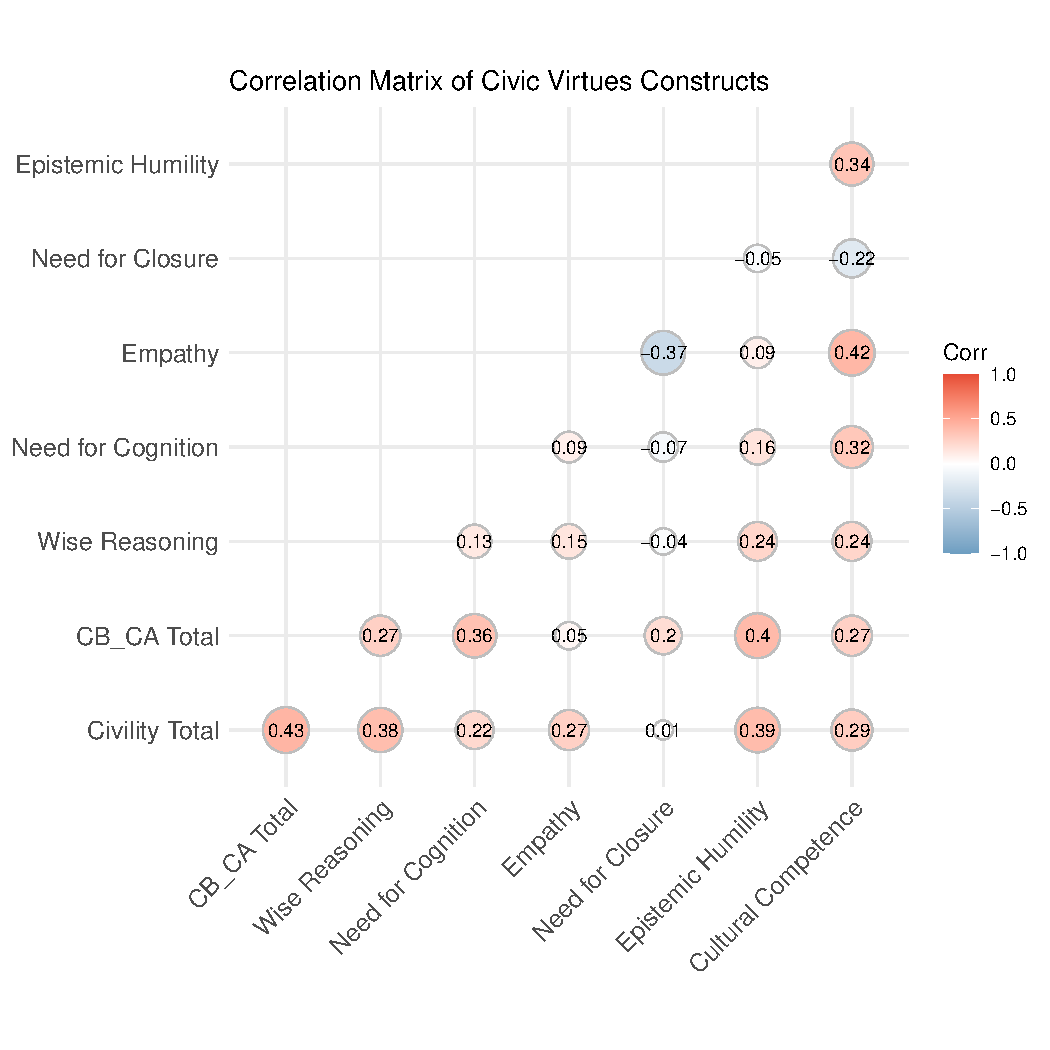
\includegraphics{civic-virtues-yyli28_files/figure-pdf/fig-correlation-plot-1.pdf}

}

\end{figure}%

The correlation matrix presented in Table~\ref{tbl-correlations} and
visualized in Figure~\ref{fig-correlation-plot} provides a comprehensive
view of these intricate relationships. \emph{CB\_CA Total} was
moderately correlated with \emph{Wise Reasoning} (r = 0.273, p = 0.011),
suggesting an interconnection between behavioral and cognitive aspects
of civic engagement. \emph{Empathy} showed notable correlations with
several constructs. It was moderately correlated with \emph{Wise
Reasoning} (r = 0.146, p = 0.181), and significantly associated with
\emph{Epistemic Humility} (r = 0.093, p = 0.393). These relationships
highlight the potential interconnectedness of psychological
characteristics related to civic virtues. \emph{Cultural Competence}
demonstrated interesting associations, including a moderate correlation
with \emph{Need for Cognition} (r = 0.32, p = 0.003). The significant
correlations, marked with asterisks in Table~\ref{tbl-correlations} (* p
\textless{} 0.05, ** p \textless{} 0.01, *** p \textless{} 0.001),
indicate the complex interplay between different psychological
constructs related to civic engagement.

\subsection{T-tests}\label{t-tests}

\begin{table}

{\caption{{Comparison of Civic Virtues Constructs between American and
International Students}{\label{tbl-t-tests}}}
\vspace{-20pt}}

[!h]
\centering
\resizebox{\ifdim\width>\linewidth\linewidth\else\width\fi}{!}{
\begin{tabular}[t]{lrrrrrrr}
\toprule
Variable & t & df & p & M (American) & SD (American) & M (International) & SD (International)\\
\midrule
Civility Total & -0.060 & 84 & 0.952 & 101.750 & 12.457 & 101.933 & 15.131\\
CB\_CA Total & 0.794 & 84 & 0.430 & 72.946 & 14.916 & 70.367 & 13.265\\
Wise Reasoning & -0.285 & 84 & 0.777 & 76.304 & 13.622 & 77.133 & 11.349\\
Need for Cognition & 0.133 & 84 & 0.895 & 21.750 & 3.684 & 21.633 & 4.255\\
Empathy & 0.943 & 84 & 0.348 & 29.679 & 3.454 & 28.900 & 3.994\\
\addlinespace
Need for Closure & 0.703 & 84 & 0.484 & 58.571 & 12.823 & 56.600 & 11.530\\
Epistemic Humility & 0.257 & 84 & 0.798 & 94.786 & 12.036 & 94.033 & 14.521\\
Cultural Competence & 0.610 & 84 & 0.544 & 34.375 & 3.840 & 33.767 & 5.328\\
\bottomrule
\end{tabular}}

\end{table}

\begin{figure}[H]

\caption{Comparison of Civic Virtues Constructs between American and
International Students}

{\centering 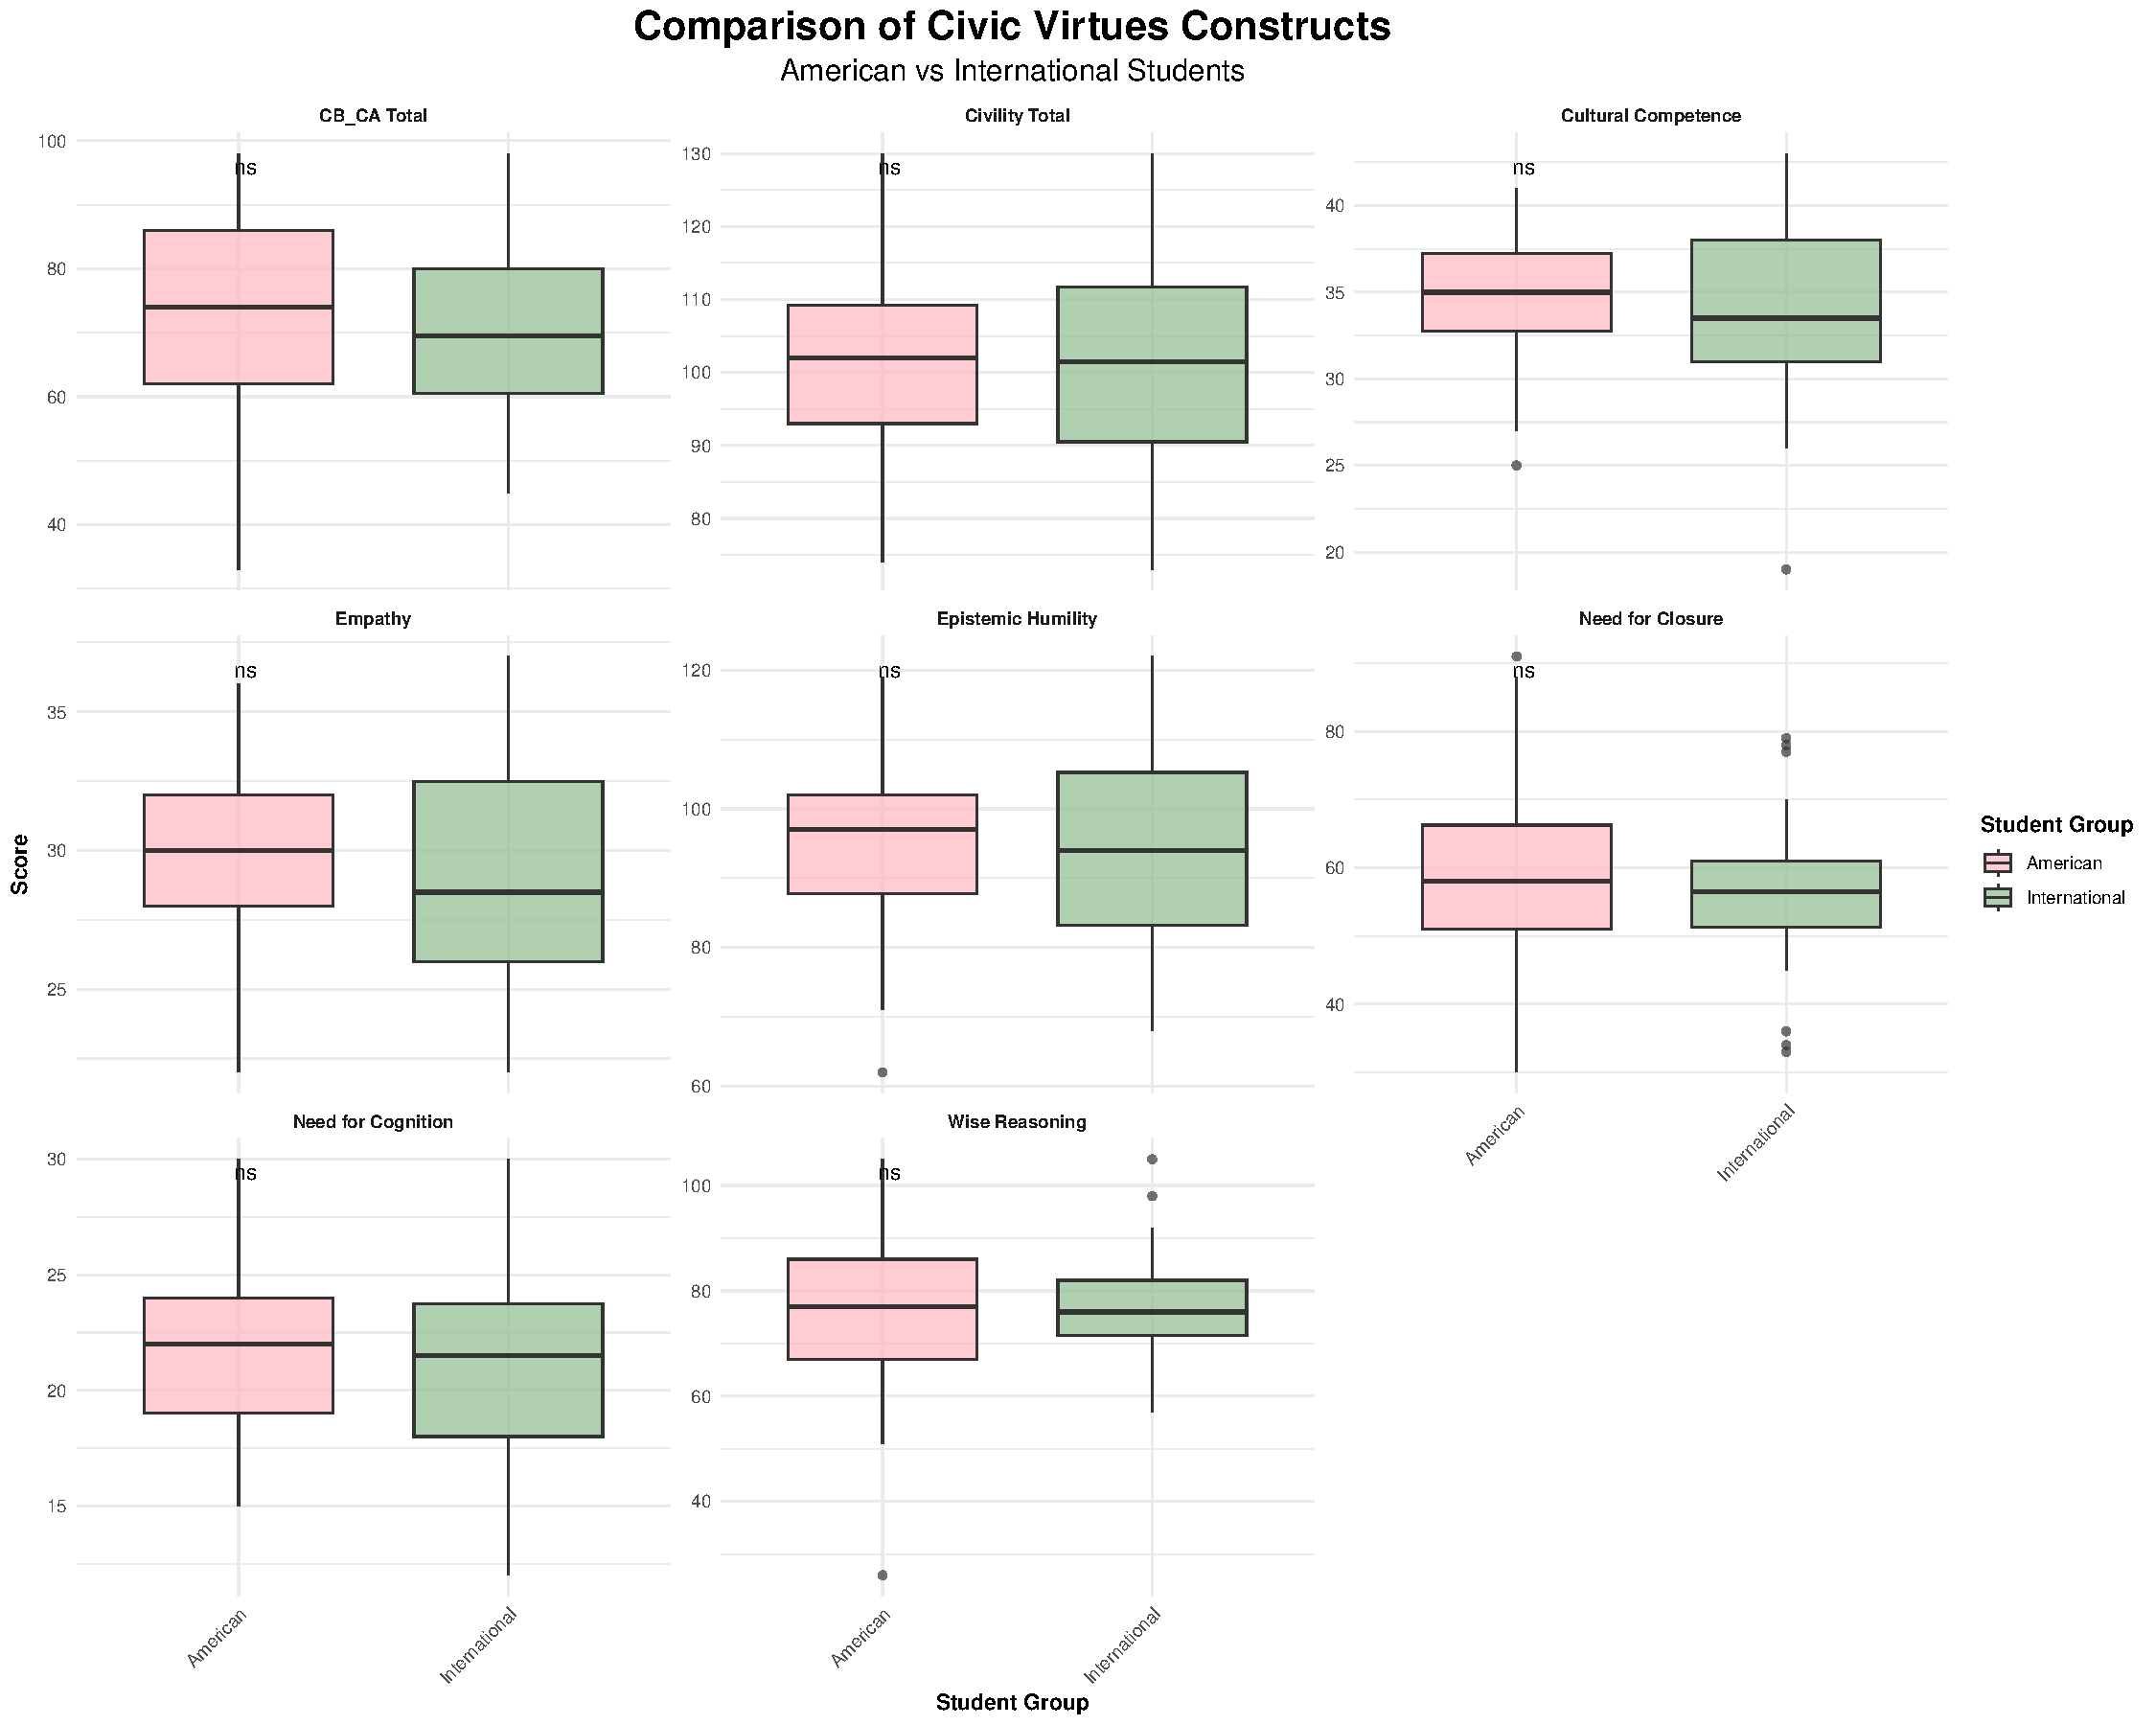
\includegraphics{civic-virtues-yyli28_files/figure-pdf/t-test-viz-1.pdf}

}

\end{figure}%






\end{document}
